\cotefile{156-9}
\scanpage{82}
\mspage{78}
% archive sheet number: 81

b) $\forall S\in\Sigma$, posant $\unsure{\beta|B}(S)=\{x\in E\mid\sigma(x)\leq S\}$, on a
\[
\deleted{S=\operatorname{Sup}(\{\sigma x\mid x\in\unsure{)|E}}
\qquad S=\operatorname{Sup}_{x\in\beta(S)}\sigma x
\]
% slanted
\margin{Cette condition \unsure{peut} s'exprimer en disant que $\sigma(E)=\Sigma'$ est une ``\uline{partie dense}'' de l'ens. \uline{ordonné} $\Sigma$, i.e. $\forall S\in\Sigma$, on a $S=\operatorname{Sup}_{\substack{x\in\Sigma'\\x\leq S}}x$.}

(Donner aussi la formulation \deleted{\unsure{symétrique}}\inserted{\unsure{symétrique} b') p.\,83})

De plus, quand ces conditions sont \unsure{satisfaites}, la \unsure{bij.} $\unsure{\alpha|\varphi}$ est uniquement déterminée.
\margin{\uline{NB} Expliciter la formule pour $\alpha$, et pour l'application inverse $\beta$.}

\uline{Dém.} La \unsure{néc.} de a) b) \unsure{évidente}, prouvons la suffisance. Utilisant a), on va déjà construire une application
\[
\alpha:\Sigma_E\longrightarrow\Sigma,
\]
en posant pour $\forall\unsure{A|\mathbb{A}|\mathscr{A}}\in\Sigma_E$
\[
\alpha(A)=\operatorname{Sup}_{x\in A}\sigma(x)
\]
Il est clair que cette application est croissante, et par b) elle est surjective, \deleted{\unsure{du|$\forall$}} au moins si on prouve que $\beta(S)$ dans b) est $\in\Sigma_E$. Soit $S'=\unsure{\complement|C|\ell|l}S$, et considérons $\beta(S')$, il suffit de voir que
\[
\beta(S)=\unsure{\operatorname{Comp}^{\circ}|\operatorname{Comp}^{o}}(\beta(S'))
\]
i.e. que pour $x\in E$, on a
\[
\underset{\text{i.e. }\sigma(x)\leq S}{x\in\beta(S)}
\quad\Longleftrightarrow\quad
x\mathrel{|{\circ}|}\beta(S')
\quad\underset{\text{(\unsure{par|pr} a)}}{\text{i.e.}}\quad
\sigma(x)\mathrel{|{\circ}|}\underset{S'_0}{\underset{\begin{tikzpicture}[baseline=0pt]\draw (0,0.08)--(0,0)--(1.8,0)--(1.8,0.08);\end{tikzpicture}}{\sigma(\beta(\unsure{S'|S}))}}
\]
Mais $\sigma(x)\mathrel{|{\circ}|}S'_0\Longleftrightarrow\sigma(x)\mathrel{|{\circ}|}\operatorname{Sup}S'_0$, et comme $\operatorname{Sup}S'_0=S'$, cela équivaut à $\sigma(x)\mathrel{|{\circ}|}S'$ ou $\sigma(x)\leq S$, OK.

\scanpage{83}
\mspage{79}
% archive sheet number: 82

En fait, on a \inserted{donc} construit une application
\diagram{\begin{tikzcd}[ampersand replacement=\&]
\Sigma \arrow[r,phantom,"{\overset{\unsure{\beta|B}}{\unsure{\longrightarrow|{-}}}}"{description}] \& \Sigma_E
\end{tikzcd}}
visiblement croissante, telle que
\[
\unsure{\alpha|\varphi}\beta=\operatorname{id}_{\Sigma}.
\]
De plus, on vient de voir qu'elle est compatible \unsure{à|:} $\unsure{\complement|C|\ell|l}$. Pour achever la dém, il suffit de voir que
\[
\inserted{\beta\alpha}\deleted{\unsure{\beta\alpha\beta|\beta\alpha}}=\operatorname{id}_{\Sigma_E},
\]
car alors $\alpha$ et $\beta$ sont des \deleted{applications \unsure{inv.}}\inserted{iso. d'ens ordonnés} \deleted{\unsure{inv.} l'une de l'autre, \unsure{croi.}}\inserted{inverses l'une de l'autre, et (comme} on voit sur $\beta$) compatibles \unsure{à|:} $\complement$.

Soit donc $\unsure{A|\mathbb{A}|\mathscr{A}}\in\Sigma_E$, $A'=\unsure{\operatorname{comp}^{\circ}|\operatorname{comp}^{o}}(A\unsure{)}$, alors les $\sigma(x)$ et $\sigma(x')$ $(x\in A,\ x'\in A')$ sont disjoints\inserted{(par a))}, donc leurs $\operatorname{Sup}$ $\alpha(A)$, $\alpha(A')$ le sont aussi\deleted{\unsure{(par a))}}. \deleted{Considérons}
\[
\deleted{\beta\alpha(A)=\{x\in E\mid\sigma(x)\leq\alpha(A)\}}
\quad\deleted{\text{\unsure{Consid il s'ensuit}}}
\]
i.e.
\[
\alpha(A)\leq\complement\alpha(A'),\quad\text{d'où}
\]
\deleted{\unsure{on a}}
\[
\beta(\alpha(A))\leq\beta\complement\alpha(A')=\complement\beta(\alpha(A')),\quad\text{i.e.}
\]
\diagram{\begin{tikzcd}[ampersand replacement=\&,column sep=small,row sep=small]
\beta\alpha(A) \arrow[d,phantom,"\leq"{description,rotate=90}] \& \mathrel{|{\circ}|} \& \beta\alpha(A'). \arrow[d,phantom,"\leq"{description,rotate=90}] \\
A \& \& A'
\end{tikzcd}}
Mais cela implique
\[
A=\beta\alpha(A),\quad A'=\beta\alpha(A'),
\]
par le

\uline{Lemme} Soit $\Sigma$ un \unsure{spotos|spatos} ($\Sigma_E$ en \unsure{l'occurrence}), soient $A\leq B$, $A'\leq B'$ avec $\deleted{\unsure{A}}B\mathrel{|{\circ}|}B'$, et $A'=\complement A$. Alors $A=B$, $A'=B'$.

En effet, on a $A\leq B\leq\complement B'\leq\complement A'=A$, donc \unsure{tous les|toutes les} $\leq$ sont des \unsure{égalités}.

\scanpage{84}
\mspage{80}
% archive sheet number: 83

Il reste à voir l'unicité de $\unsure{\alpha|\varphi}$, qui est immédiate, vu que $\deleted{\unsure{\forall}}\unsure{A|\mathbb{A}|\mathscr{A}}\in\Sigma_E$ est le $\sup$ des $\sigma_E(x)$ qu'il majore (i.e. tels que $x\in A$ \ldots), \deleted{et $\alpha$ doit \unsure{ce}} d'où forcément
\[
\alpha(A)=\operatorname{Sup}_{x\in A}\underbrace{\alpha(\sigma_E(x))}_{\sigma(\unsure{x|*})}\unsure{=|\equiv}\operatorname{Sup}_{x\in A}\sigma(x)
\qquad\text{\unsure{qed}}
\]

\deleted{\uline{Corollaire} Soit $(E,\inserted{\unsure{\leq^{\circ}|\leq},}\mathrel{|{\circ}|})$ un \unsure{disjoncteur} ordonné, $E_0$ une partie très dense de $E$}

\uline{Corollaire\unsure{!|1}} Soit $\deleted{E}(E,\mathrel{|{\circ}|}_E)$ un \unsure{disjoncteur}, $E'$ une partie de $E$, $\mathrel{|{\circ}|}_{E'}$ la relation induite. Conditions équivalentes:

(i) L'image $\deleted{\unsure{E'}}\sigma_E(E')$ de $E'$ dans $\Sigma_E$ est dense, i.e. tout $S\in\Sigma_E$ est le $\sup$ de l'ens. des éléments de $\sigma_E(E')$ qu'il majore.

(ii) \deleted{\unsure{L'}} L'application
\[
S\longrightarrow S\cap E',\quad\Sigma_E\unsure{{-}|\longrightarrow|\longmapsto}\unsure{\mathscr{P}|\mathcal{P}|\mathfrak{P}}(E')
\]
\deleted{applique $\Sigma_E$ dans $\Sigma_{E'}$, et induit une}
\inserted{est \uline{\unsure{injection|surjection}}}
(NB elle induit alors \unsure{$=$|$\simeq$} un iso
\[
\varphi:\Sigma_E\longrightarrow\Sigma_{E'}).
\]
\deleted{\unsure{(NB. ce sera} $=$ un iso)}

(iii) L'application
\[
\begin{aligned}
\psi:\Sigma_{E'}&\longrightarrow\Sigma_E\\
S'&\longmapsto\unsure{\operatorname{supp}^{\circ}_E|\operatorname{supp}^{o}_E}(S')
\end{aligned}
\]
est \unsure{surjective|bijective} (NB ce sera \unsure{$=$|$\simeq$} un iso)

% slanted
\margin{$\longleftarrow$ \unsure{permuter} avec (v) \deleted{\unsure{comme (i bis)}}}
(iv) $E'$ est \uline{dense} dans $E$ pour la relation d'\inserted{pré}ordre canonique de $E$ (induite de celle de $\Sigma_E$ via $\sigma_E$).

\scanpage{85}
\mspage{81}
% archive sheet number: 84

\inserted{(\deleted{\unsure{iv bis|iv}}) $\forall x,y\in E$, si $\forall x',y'$ avec $x'\leq x$, $y'\leq y$, on a $x'\mathrel{|{\circ}|}y'$, alors $x\mathrel{|{\circ}|}y$. (La relation $\leq$ est la relation d'ordre canonique)}

Dans ces conditions, les applications $\varphi$, $\psi$ sont inverses l'une de l'autre, et sont des isomorphismes de \unsure{spotos|spatos}.

\uline{Dém} $(i)\Longleftrightarrow(iv)$, \inserted{\unsure{évident}}, compte tenu que (iv) signifie aussi que $\sigma(E')$ est dense dans $\sigma(E)$, pour l'ordre induit par $\Sigma_E$. (Attention, ``dense'' ici au sens de la relation d'ordre, qui \deleted{\unsure{n'est pas}} \unsure{notion|n'est} \unsure{pas|fort} \unsure{pris|prise} au sens de la topologie associée à l'ordre; mais on a néanmoins transitivité de la notion de densité, grâce à l'associativité des $\sup$.)

$(i\deleted{\unsure{v}})\Longrightarrow(v)$ est encore une assertion sur $\underset{\begin{tikzpicture}[baseline=0pt]\draw (0,0.08)--(0,0)--(1.9,0)--(1.9,0.08);\end{tikzpicture}}{\sigma(E')\subset\sigma(E)}\subset\Sigma$, et immédiate, car dans $\Sigma$, \deleted{\unsure{En}} Si $x=\operatorname{Sup}x_i$, $y=\operatorname{Sup}y_j$, $x_i\mathrel{|{\circ}|}y_j$ $\forall i,j$, alors $x\mathrel{|{\circ}|}y$.

$(v)\Longrightarrow(iv)$ \deleted{Soit $S\in\Sigma_E$,} On se place encore dans $\Sigma$ avec $\sigma(E')\subset\sigma(E)\subset\Sigma$. Soit \deleted{$S=\sigma(x)\in\sigma(E)$.} $\inserted{\unsure{\xi|\zeta}}\deleted{\unsure{S}}\in\sigma(E)$. \deleted{Dire que} Considérons l'ens $S'_0$ des $\xi'\in\sigma(E')$ tels que $\xi'\leq\xi$. Je dis que
\[
\xi=\operatorname{Sup}_{\deleted{\unsure{\xi'\in S'_0}}}\xi'
\]
Mais (cf Lemme \inserted{\unsure{ci dessous|ci-dessus|ci-dessous}}) cela signifie aussi que pour tout $\deleted{\unsure{S|S'}}\unsure{\eta|y|\theta}\in\sigma(E)$, on a $\unsure{S'_0|\xi'}\mathrel{|{\circ}|}\eta$, on a $\xi\mathrel{|{\circ}|}\eta$. Considérons donc $T'=\{\eta'\in\sigma(E')\mid\eta'\leq\eta\}$. On a donc $\xi'\mathrel{|{\circ}|}\eta'$ pour $\xi'\in\unsure{S'|S'_0}$, $\eta'\in T'$. Par hypo, cela implique $\xi\mathrel{|{\circ}|}\eta$, OK.

\scanpage{86}
\mspage{82}
% archive sheet number: 85

\uline{Lemme} Soient $\Sigma$ un \unsure{spotos|spatos}, $E$ une partie dense (cf \ldots), $S'$ une partie de $\Sigma$, formée d'éléments majorés par un $\unsure{\xi|\zeta}\in\Sigma$, donc i.e. $\operatorname{Sup}S'\leq\xi$. Pour qu'on ait $\operatorname{Sup}S'=\xi$, il f. et s. que pour $\forall\unsure{\eta|y|\theta}\in E$, \deleted{tel que}
\[
\deleted{S'\mathrel{|{\circ}|}\eta\Rightarrow.}\qquad
S'\mathrel{|{\circ}|}\eta\Longrightarrow\xi\mathrel{|{\circ}|}\eta
\]

\uline{Dém} \unsure{au|du} Lemme. On sait déjà que si $\operatorname{Sup}S'=\xi$, alors $\forall\eta\in\Sigma$, on a
\[
S'\mathrel{|{\circ}|}\eta\Longleftrightarrow\xi\mathrel{|{\circ}|}\eta.
\]
En sens inverse, \deleted{\unsure{supposons que On}}\inserted{Supposons que}
\deleted{\unsure{veut prouver|on prouve} $\operatorname{Sup}(S')=\xi$ i.e. $\xi\leq\operatorname{Sup}S'$,}
\deleted{on aura $\unsure{\complement|C|\ell|l}\xi\geq\operatorname{Inf}$}
\[
\forall\eta\in E,\qquad
\underbrace{S'\mathrel{|{\circ}|}\eta}_{\substack{\text{\unsure{i.e.|i.e} }\deleted{\unsure{S'\leq}}\\\eta\leq\operatorname{Inf}_{\xi'\in S'}\complement(\xi')}}
\Longrightarrow
\underbrace{\xi\mathrel{|{\circ}|}\eta}_{\substack{\text{\unsure{i.e.|ie}}\\\eta\leq\complement(\xi)}}
\]
À cause de la densité, on en conclut
\[
\operatorname{Inf}_{\xi'\in S'}\complement(\xi')\leq\complement(\xi)
\]
D'où
\[
\unsure{\eta|\xi|\zeta}\leq\operatorname{Sup}_{\xi'\unsure{=|\in}S'}\xi',\qquad\text{\uline{qed}}
\]

Ainsi, les conditions (i) (iv) (v) de la prop.\unsure{2|?} sont équivalentes. Compte tenu de prop. 1, la condition (i) implique que l'application composée $E'\subset E\mathbin{-}\Sigma_E$ permet d'identifier $\Sigma_E$ à $\Sigma_{E'}$. Cette identification est visiblement donnée par (ii)

\scanpage{87}
\mspage{83}
% archive sheet number: 86

(cf construction de l'application $\unsure{\beta|B}$ de prop. 2), et au sens inverse par (iii) (application $\unsure{\alpha|\varphi}$ de prop. 2). Donc, (i) (ou ses voisines (iv), (v)) implique (ii), (iii) sous forme plus forte (iso. de \unsure{spotos|spatos}). Il reste à prouver que (ii) ou (iii) implique \inserted{déjà} (i).

Mais que (iii) (\unsure{et|i.e.} simplement la \uline{surjectivité} de $\psi$) implique (i), est clair. Donc (iii) équivaut aux autres conditions. Reste à voir que (ii) implique (i). Cela équivaut au corollaire suivant, appliqué à $E'\mathbin{-}\Sigma_E$

\uline{Corollaire 2} Soient $E$ un \unsure{disjoncteur}, $\Sigma$ un spotos, $\sigma:E\longrightarrow\Sigma$ une application. Alors la condition b) de la prop 2 est équivalente (moyennant a)) à la condition suivante:
\margin{\figure{\begin{tikzpicture}[x=1mm,y=1mm]\draw[->] (0,28)--(0,0);\end{tikzpicture}}}

b') L'application $S\longrightarrow\beta(S)$ de $\Sigma$ dans $\unsure{\mathscr{P}|\mathcal{P}|\mathfrak{P}}(E)$ applique $\Sigma$ dans $\Sigma_E$, et est \deleted{bijective}\inserted{injective}.
\margin{\figure{\begin{tikzpicture}[x=1mm,y=1mm]\draw (0,12)--(0,0);\end{tikzpicture}}}

On a vu dans la démonstration que b) $\Longrightarrow$ b'). Prouvons que b') $\Longrightarrow$ b). Considérons, pour $S\in\Sigma$ fixé, $S'=\operatorname{Sup}\sigma(\beta(S))\unsure{(}\leq S\unsure{)}$. Il est clair que $\beta(S)=\beta(S')$, donc $S=S'$, puisque $\beta$ est injectif qed

\scanpage{88}
\mspage{84}
% archive sheet number: 87

\uline{Corollaire \unsure{5|3}} Soient $(E,\leq,\mathrel{|{\circ}|})$ un \unsure{disjoncteur} \unsure{préordonné}, et soit $E'$ une partie de $E$ qui est ``dense'' dans le sens suivant
\[
\forall x,y\in E,\quad\deleted{\unsure{\forall}}\quad
E'_{\leq x}\mathrel{|{\circ}|}E'_{\leq y},\quad\Longrightarrow x\mathrel{|{\circ}|}y.
\]
Alors
\diagram{\begin{tikzcd}[ampersand replacement=\&,column sep=large]
\Sigma_{E'} \arrow[r,shift left=1ex,"\underset{\sim}{\unsure{\psi|\varphi}}"] \& \Sigma_E \arrow[l,shift left=1ex,"\varphi","\sim"']
\end{tikzcd}}
iso. inverses l'un de l'autre, donnés par
\[
\begin{aligned}
\psi(\unsure{A'|\mathbb{A}'|\mathscr{A}'})&=\unsure{\operatorname{supp}^{\circ}_E|\operatorname{supp}^{o}_E}(A')\\
\varphi(A)&=A\cap E'.
\end{aligned}
\]

On applique cor. 1, critère (v), en notant que la condition de densité ici est plus forte \unsure{à|a} priori que celle dans (v).

\figure{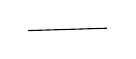
\begin{tikzpicture}[x=1mm,y=1mm]\draw (0,0)--(10,.3);\end{tikzpicture}}

\deleted{\unsure{Les}} \uline{\unsure{Correspondances} entre \inserted{disjoncteurs et entre} Spotos.} $\deleted{\unsure{\Sigma}}$

\deleted{\unsure{Les|des}} \uline{Analogie} Soient $E,E'$ deux ensembles, \deleted{\unsure{i.e.}} ou encore disjoncteurs triviaux. Une ``corr'' (ou ``relation'' \inserted{$R$}) entre $E,E'$ peut \unsure{être|etre} \unsure{interprétée} comme une application
\[
\unsure{\alpha|\varphi}:E\unsure{{-}|\longrightarrow}\unsure{\mathscr{P}|\mathcal{P}|\mathfrak{P}}(E')
\qquad(x\unsure{\longmapsto|{\mid}{-}}R(x))
\]

\scanpage{89}
\mspage{85}
% archive sheet number: 88

et elle se prolonge aussitôt en une application
\[
\unsure{\alpha_*|\varphi_*|\alpha_{\times}}\text{ ou }\bar\alpha:
\unsure{\mathscr{P}|\mathcal{P}|\mathfrak{P}}(E)\unsure{{-}|\longrightarrow}\mathscr{P}(E')
\qquad\unsure{A|\mathbb{A}|\mathscr{A}}\mathbin{-}\bigcup_{x\in A}\alpha(x)
\]
% slanted
\margin{J'écris $\bar\alpha$ en pensant à des \unsure{parties} des ensembles $E,E'$ et $\alpha_*$ en pensant à une application entre \unsure{spotos|spatos}.}

Cette application $\bar\alpha$ commute aux $\operatorname{Sup}$ quelconques\inserted{(donc est croissante)}, et inversement, toute application $\varphi:\mathscr{P}(E)\mathbin{-}\mathscr{P}(E')$ qui a cette propriété, s'écrit de façon unique sous la forme $\alpha_*$, puisque $\deleted{\unsure{\forall}}A\in\mathscr{P}(E)$, on a
\[
A=\operatorname{Sup}_{x\in A}\{x\}\quad\text{donc}\quad
\varphi(A)=\operatorname{Sup}_{x\in A}\underset{\alpha(x)\,{}^{\text{``\unsure{def|déf}}}}{\underset{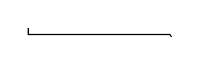
\begin{tikzpicture}[baseline=0pt]\draw (0,0.08)--(0,0)--(1.8,0)--(1.82,-0.03);\end{tikzpicture}}{\varphi(\{x\})}}
\]
% slanted
\margin{\unsure{Compatibilité} avec la \unsure{composition} des \unsure{correspondances}\figure{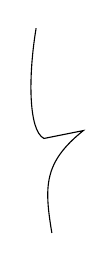
\begin{tikzpicture}[x=1mm,y=1mm]\draw (0,26) .. controls (-1,20) and (-1,13) .. (1,12) -- (6,13) .. controls (1,9) and (1,6) .. (2,0);\end{tikzpicture}}}

Nous allons interpréter l'a\deleted{\unsure{pp|p}} correspondance symétrique, ou transposée, $\unsure{\beta|B}$ de $\alpha$, en termes de
\[
\beta_*\text{ ou }\bar\beta:\mathscr{P}(E')\longrightarrow\mathscr{P}(E),
\]
en \deleted{\unsure{tant}} termes des spotos $\mathscr{P}(E)$, $\mathscr{P}(E')$, en notant que
% Left-hand label as on the scan.
\begingroup
\makeatletter\tagsleft@true\makeatother
\[
\left\{\begin{aligned}
&\forall A\in\mathscr{P}(E),\ A'\in\mathscr{P}(E')\quad\text{on a}\\
&\alpha_*(A)\mathrel{|{\circ}|}A'\Longleftrightarrow A\mathrel{|{\circ}|}\beta_*(A')
\end{aligned}\right.
\tag*{\unsure{a)|b)}}
\]
\endgroup
En effet, le premier \unsure{mb|m.b.} s'écrit
\[
\begin{aligned}
&\deleted{\unsure{\forall x\in A,}}\forall x'\in A',\quad\text{on a }x'\notin\bar\alpha(A)\quad\text{i.e. }\unsure{\nexists|\exists}x\in A\\
&\text{avec }x'\in\unsure{\alpha|\bar\alpha}(x)\quad\text{i.e. }(x,x')\in R
\end{aligned}
\]
ou encore
\[
\forall\unsure{x'|x}\in A,\ x'\in A'\quad\text{on a }(x,x')\notin R\quad\text{i.e. }(x,x')\in\bar R
\]
